The history of any physical field is interesting in several ways. Physical questions usually start with one or more observations, the \textit{what}, and then the urge to understand \textit{why}. In science, \textit{why} is of course the question we ideally want to answer, but in many cases that is not achievable at first. An example is the statement of Kepler's three laws of planetary motion. Kepler had observations that he confirmed were indeed correct, but he did not know \textit{why} the planets behave like they do. Some 50 years later, Newton explained Kepler's three laws by his universal law og gravitation. This is the beauty of science, the \textit{why} is not required, just desired.\\
Another interesting part of the history is the amount of available information at the time of discoveries, which strongly affects their ability to develop new theories. Newton needed to create a theory that were in agreement with Kepler's laws, and Kepler needed his laws to agree with the observations that were done. In this chapter, we will briefly discuss some of the discoveries and questions in fluid mechanics that lead up to our current knowledge of the field. 
\section{The beginning in Greece}
The first scientific descriptions of fluid mechanics dates back to Aristotle (384-322 B.C.) when he identified the continuum and dynamic drag in fluids \cite{anderson1998history}. He wrote
\begin{aquote}{Aristotle by Lysippus}
The continuous may be defined as that which is divisible into parts which are themselves divisible to infinity, as a body which is divisible in all ways. Magnitude divisible in one direction is a line, in three directions a body. And magnitudes which are divisible in this fashion are continuous. 
\end{aquote}
The idea of continuum is fundamental in most fluid mechanics theories and is a rather abstract concept that makes the mathematics work out beautifully. At the time of Aristotle, the mathematical framework was not yet established, so it was an impressive contribution to the field. The more intuitive drag force was described as
\begin{aquote}{Aristotle by Lysippus}
It is impossible to say why a body that has been set in motion in a vacuum should ever come to rest. Why, indeed, should it come to rest at one place rather than another. As a consequence, it will either necessarily stay at rest, or if in motion, will move indefinitely unless some obstacle comes into collision with it.
\end{aquote}
For fluids in movement, the obstacle is the thing creating the drag force preventing the fluid to move freely. About a hundred years later, Archimedes (287-212 B.C.) published \textit{On Floating Bodies} where he discussed what is now known as \textit{Archimedes' principle} that states
\begin{aquote}{Archimedes of Syracuse}
Any object, wholly or partially immersed in a fluid, is buoyed up by a force equal to the weight of the fluid displaced by the object.
\end{aquote}
Even today, more than 2000 years later, every high school student taking a physics course learn about Archimedes' principle. It is a simple and intuitive, yet remarkably powerful, statement that can easily be derived using Newtonian mechanics. 

\section{The Euler equations and the Navier-Stokes equations}
With the concept of continuum, we think that each point in space has well defined physical properties like temperature, density and momentum. In 1757, Euler published what's called the \textit{Euler equations} by applying conservation of mass, momentum and energy to a small volume element $\dm V$. It is a set of differential equations describing how the fluid velocity field changes in time and space. The conservation laws can be written as
\begin{align}
	\dpart{\rho_m}{t} + \nabla\cdot (\rho_m\vec u) &= 0 \qquad \text{mass}\\
	\dpart{\rho_m \vec u}{t} + \nabla \cdot (\vec u \otimes (\rho_m\vec u)) + \nabla P &= 0\qquad \text{momentum}\\
	\dpart{E}{t} + \nabla\cdot (\vec u(E + p)) &= 0\qquad \text{energy},
\end{align}
where $\rho_m$ is the mass density, $\vec u(\vec x, t)$ is the velocity field, $E$ is the total energy per unit volume, $\otimes$ is the tensor product and $P(\vec x, t)$ is the pressure field. These can be combined to one vector equation, but the idea of conservation laws are more clear when they are separated. In the original paper, Euler only derived the first two equations, but the full set is usually referred to as the Euler equations. They describe the motion of fluids with negligible viscosity which is a decent approximation for many fluids.\\
About 80 years later, in the 1840s, Sir George Stokes published the Navier-Stokes equations (NSE) which can be seen as an extension of the Euler equations where effects caused by the viscosity of the fluid are included \cite{batchelor2000introduction}. The Navier-Stokes equations for an incompressible fluid can be written as one vector equation
\begin{align}
	\label{eq:nse_incompressible}
	\rho_m \frac{D\vec u}{Dt} = \rho_m \vec F - \nabla p + \mu\nabla^2\vec u,
\end{align}
where $\vec F$ is an external force (i.e. gravity or an electrostatic field), $\mu$ is the viscosity and $D/Dt$ is the material derivative defined as
\begin{align}
	\frac{D}{Dt} = \dpart{}{t} + \vec u\cdot \nabla.
\end{align}
These are also a set of coupled non-linear differential equations that can be seen as one vector differential equation. It has quite a few interesting analytically solvable solutions, but for most real systems, the geometry confining the fluid is so complex that it is usually solved on computers. The equation above is valid for incompressible fluids where the mass-conservation equation is written as (constant density)
\begin{align}
	\nabla\cdot \vec u = 0,
\end{align}
which is a good approximation for many liquids. However, most gases are compressible, and the more general NSE including theses effects is given as
\begin{align}
	\rho_m \frac{D\vec u}{ Dt} = \rho_m \vec F - \nabla p + \mu\nabla^2\vec u + \mu\nabla(\nabla\cdot \vec u),
\end{align}
where we notice the extra term compared to equation \eqref{eq:nse_incompressible}. When solving the NSE, one has to provide boundary conditions to get a unique solution for the system. Usually, one applies no-slip boundary conditions, i.e. that the fluid velocity is zero at the container walls. In section \ref{sec:slip_length} we discuss the effects of slip velocity and how this affects the flow properties of the fluid. 
\section{Macroflows and microflows}
When we solve the equations governing our fluid flow, we add boundary conditions defining the geometry of our system. In the 1990s H. Bau and J. Zemel (University of Pennsylvania) performed some experiments on microchannel flow in which they found clear deviations from what was expected from the theory\cite{karniadakis2005microflows}. It is useful to introduce the terms \textit{microflows} for flow in geometries where the distance between the channel walls is of micrometer size and \textit{macroflows} for larger systems (milimeter and above). Flow at microscales differ from macroscales because of effects that can be classified into four groups
\begin{itemize}
\item noncontinuum effects,
\item surface-dominated effects,
\item low Reynolds number effects, and
\item multiscale and multiphysics effects.
\end{itemize}
In this thesis, we focus on the noncontinuum effects which are briefly discussed in section \ref{sec:continuum_breakdown}, and the surface-dominated effects as the slip condition described in section \ref{sec:slip_length}. See \cite{karniadakis2005microflows} for details about the effects of low Reynolds number and multiscale and multiphysics. 
\section{The breakdown of continuum}
\label{sec:continuum_breakdown}
A fundamental assumption in the derivation of the NSE is that the space is continuous. We know that in reality, the mass of the fluid is concentrated in the very center of the atoms, but we often assume that the mass is uniformly distributed in the volume element of which the conservations laws are applied on. This is known as the \textit{continuum hypothesis} and is invalid when the \textit{mean free path} $\lambda$, the average distance a particle moves between collisions, becomes large compared to some characteristic length $L$ in the system, i.e. the diameter of a channel\cite{karniadakis2005microflows}. This property is quantified through the \textit{Knudsen number}
\begin{align}
	\text{Kn} = \frac{\lambda}{L}.
\end{align}
From the kinetic theory we can calculate the mean free path (which is done in section \ref{sec:mean_free_path_calculation})
\begin{align}
	\lambda = \frac{m}{\sqrt 2 \pi d \rho_n} = \frac{k_B T}{\sqrt 2 \pi d^2 P},
\end{align}
where $\rho_n$ is the number density and $m$ and $d$ are the mass and diameter of the particles. By inserting the ideal gas law $P = \rho_n k_BT$, we can eliminate the density and use the pressure $P$ together with the temperature $T$ instead. Here $k_B$ is of course Boltzmann's constant. For Knudsen numbers smaller than $10^{-2}$, the continuum hypthosis is valid and we can apply the Navier-Stokes equations\cite{karniadakis2005microflows}. The Knudsen number is so important that it deserves to be discussed in more detail in section \ref{sec:knudsen_number}.
\section{Atomic models}
For systems where the continuum hypothesis is invalid, we need other models describing the behaviour of the particles in our system. The first idea that might pop our minds might be to study the system at the atomic level. The physical set of rules that are controlling the atoms is of course quantum mechanics. The equations of motion and hence the dynamics of an atomic system can in principle be calculated directly from quantum mechanics by solving Schr\"{o}dinger's equation with perturbation theory. Since this requires calculating the wave function of every atom with complex atomic interactions, the size of the system needs to be very small with today's computers. An alternative, popular approach is to use a parameterized potential $U(\vec r^N)$ ($\vec r^N$ being the positions of all atoms), and calculate the forces through the gradient of $U$. Newton's equations of motion is then integrated and the dynamics of the system are determined in a classical, deterministic way where important effects from quantum mechanics can be embedded in the potential. This method is called \textit{Molecular Dynamics} and is studied in chapter \ref{chap:md}. Molecular Dynamics is orders of magnitudes faster than models solving Schr\"{o}dinger's equation, but it still needs a detailed describtion of the dynamics of every atom in the system. For many problems, this information is redundant because what's really important is the statistical properties of the system.
\section{Statistical mechanics}
We know from statistical mechanics that what dominates the macroscopic effects is the statistical behaviour of the system. One can for example derive the ideal gas law from pure statistical and combinatorial arguments with conservation of energy being the only physical concept\cite{ravndal2008statmech}. The idea is that it is the average properties of a system that are being observed wheras the actual state (i.e. all the positions and velocities of all atoms) of the system is not known, nor needed. A physical system is often described as a distribution function $f(\vec p, \vec r; t)$ yielding the probability of finding an atom, or in general a particle with position in the range $\vec r + \dm {\vec r}$ with momentum in the range $\vec p + \dm {\vec p}$ at the time $t$. The dynamics of this function is described by the Boltzmann equation which is derived in chapter \ref{chap:kinetic_theory}. From the Boltzmann equation, we can derive the results we need to describe the properties of gases which will be input parameters to a model called Direct Simulation Monte Carlo (DSMC) which is studied in chapter \ref{chap:dsmc}. 

\section{Knudsen number}
\label{sec:knudsen_number}
To get an idea of the length scales where the Knudsen number is about unity, the mean free path for helium at $T=$\unit{273}{\kelvin} and $P=1$ atm is\cite{lillestol2001generell} 
\begin{align}
	\label{eq:helium_mfp}
	\lambda_{\text{He}} = \unit{0.17}{\micro\meter} = \unit{170}{\nano\meter}.
\end{align}
This means that for systems where the channels have diameter of a few hundred nanometers, the Knudsen number is around unity, and the continuum hypothesis is invalid. 
\section{Slip velocity}
\label{sec:slip_length}
The Navier-Stokes equations need boundary conditions of the velocity field defining the geometry of which the fluid is confined in. As mentioned earlier, the simplest boundary condition is the no-slip condition where
\begin{align}
	\vec u(\vec r; t) = 0 \qquad \vec r \in \partial\Omega
\end{align}
where $\partial\Omega$ defines the boundary domain. The history of the no-slip condition is studied by Day, based on the work of Stokes in the 19th century. Stokes compared theoretical results to experiments for pendulums of different kinds and concluded that\cite{day1990no}
\begin{aquote}{Stokes, 1901}
	I shall assume, therefore, as the conditions to be satisfied at the boundaries of the fluid, that the velocity of a fluid particle shall be the same, both in magnitude and direction, as that of the solid particle with which it is in contact. The agreement of the results thus obtained with observation will presently appear to be highly satisfactory.
\end{aquote}
In Day's detailed study of the no-slip condition, he says
\begin{aquote}{Day, 1990}
	Looking back, it appears that the acceptance of a more general no-slip condition was prolonged because of experimental shortcomings, not because of a lack of the \'appropriate\' theoretical solutions to fluid flow problems.
\end{aquote}
In other words, the theoretical framework that existed already in the time of Stokes were complete enough to include both slip and no-slip solutions. In fact, Maxwell predicted slip velocity in a paper already in 1867\cite{maxwell1879stresses}, but the experiments the next 50 years seemed to more or less confirm the no-slip condition. \todo{Discuss the later experiments showing discrepancies} Klinkenberg also has a nice argument that supports the slip velocity
\begin{aquote}{L.J. Klinkenberg, 1941}
Consider a layer adjacent to the wall which is thinner than the mean free path $\lambda$ of the gas molecules, so that practically a molecule does not collide with other molecules present in this layer. At a given moment half of the gas molecules in this layer will have a component of velocity moving towards the wall; the other half in the opposite direction. The molecules moving towards the wall have had their last collision somewhere in the flowing mass, and, therefore, will have an average velocity component in the direction of flow different from zero. A part of this average velocity component will be lost in colliding with the wall. Even if the molecules lose it entirely, then still the average velocity component in the direction of flow of all the molecules contained in the layer will amount to half of the average velocity component of the molecules moving towards the wall. The gas in the layer, therefore, will have a finite rate of flow.
\end{aquote}
It is convenient to introduce the concept of \textit{slip length} $l_s$ to be able to quantify the slip velocity. Slip length is defined as the distance into the wall we would have to extrapolate a velocity profile for it to reach zero value, see figure \ref{fig:slip_length}.
\begin{figure}[h]
\begin{center}
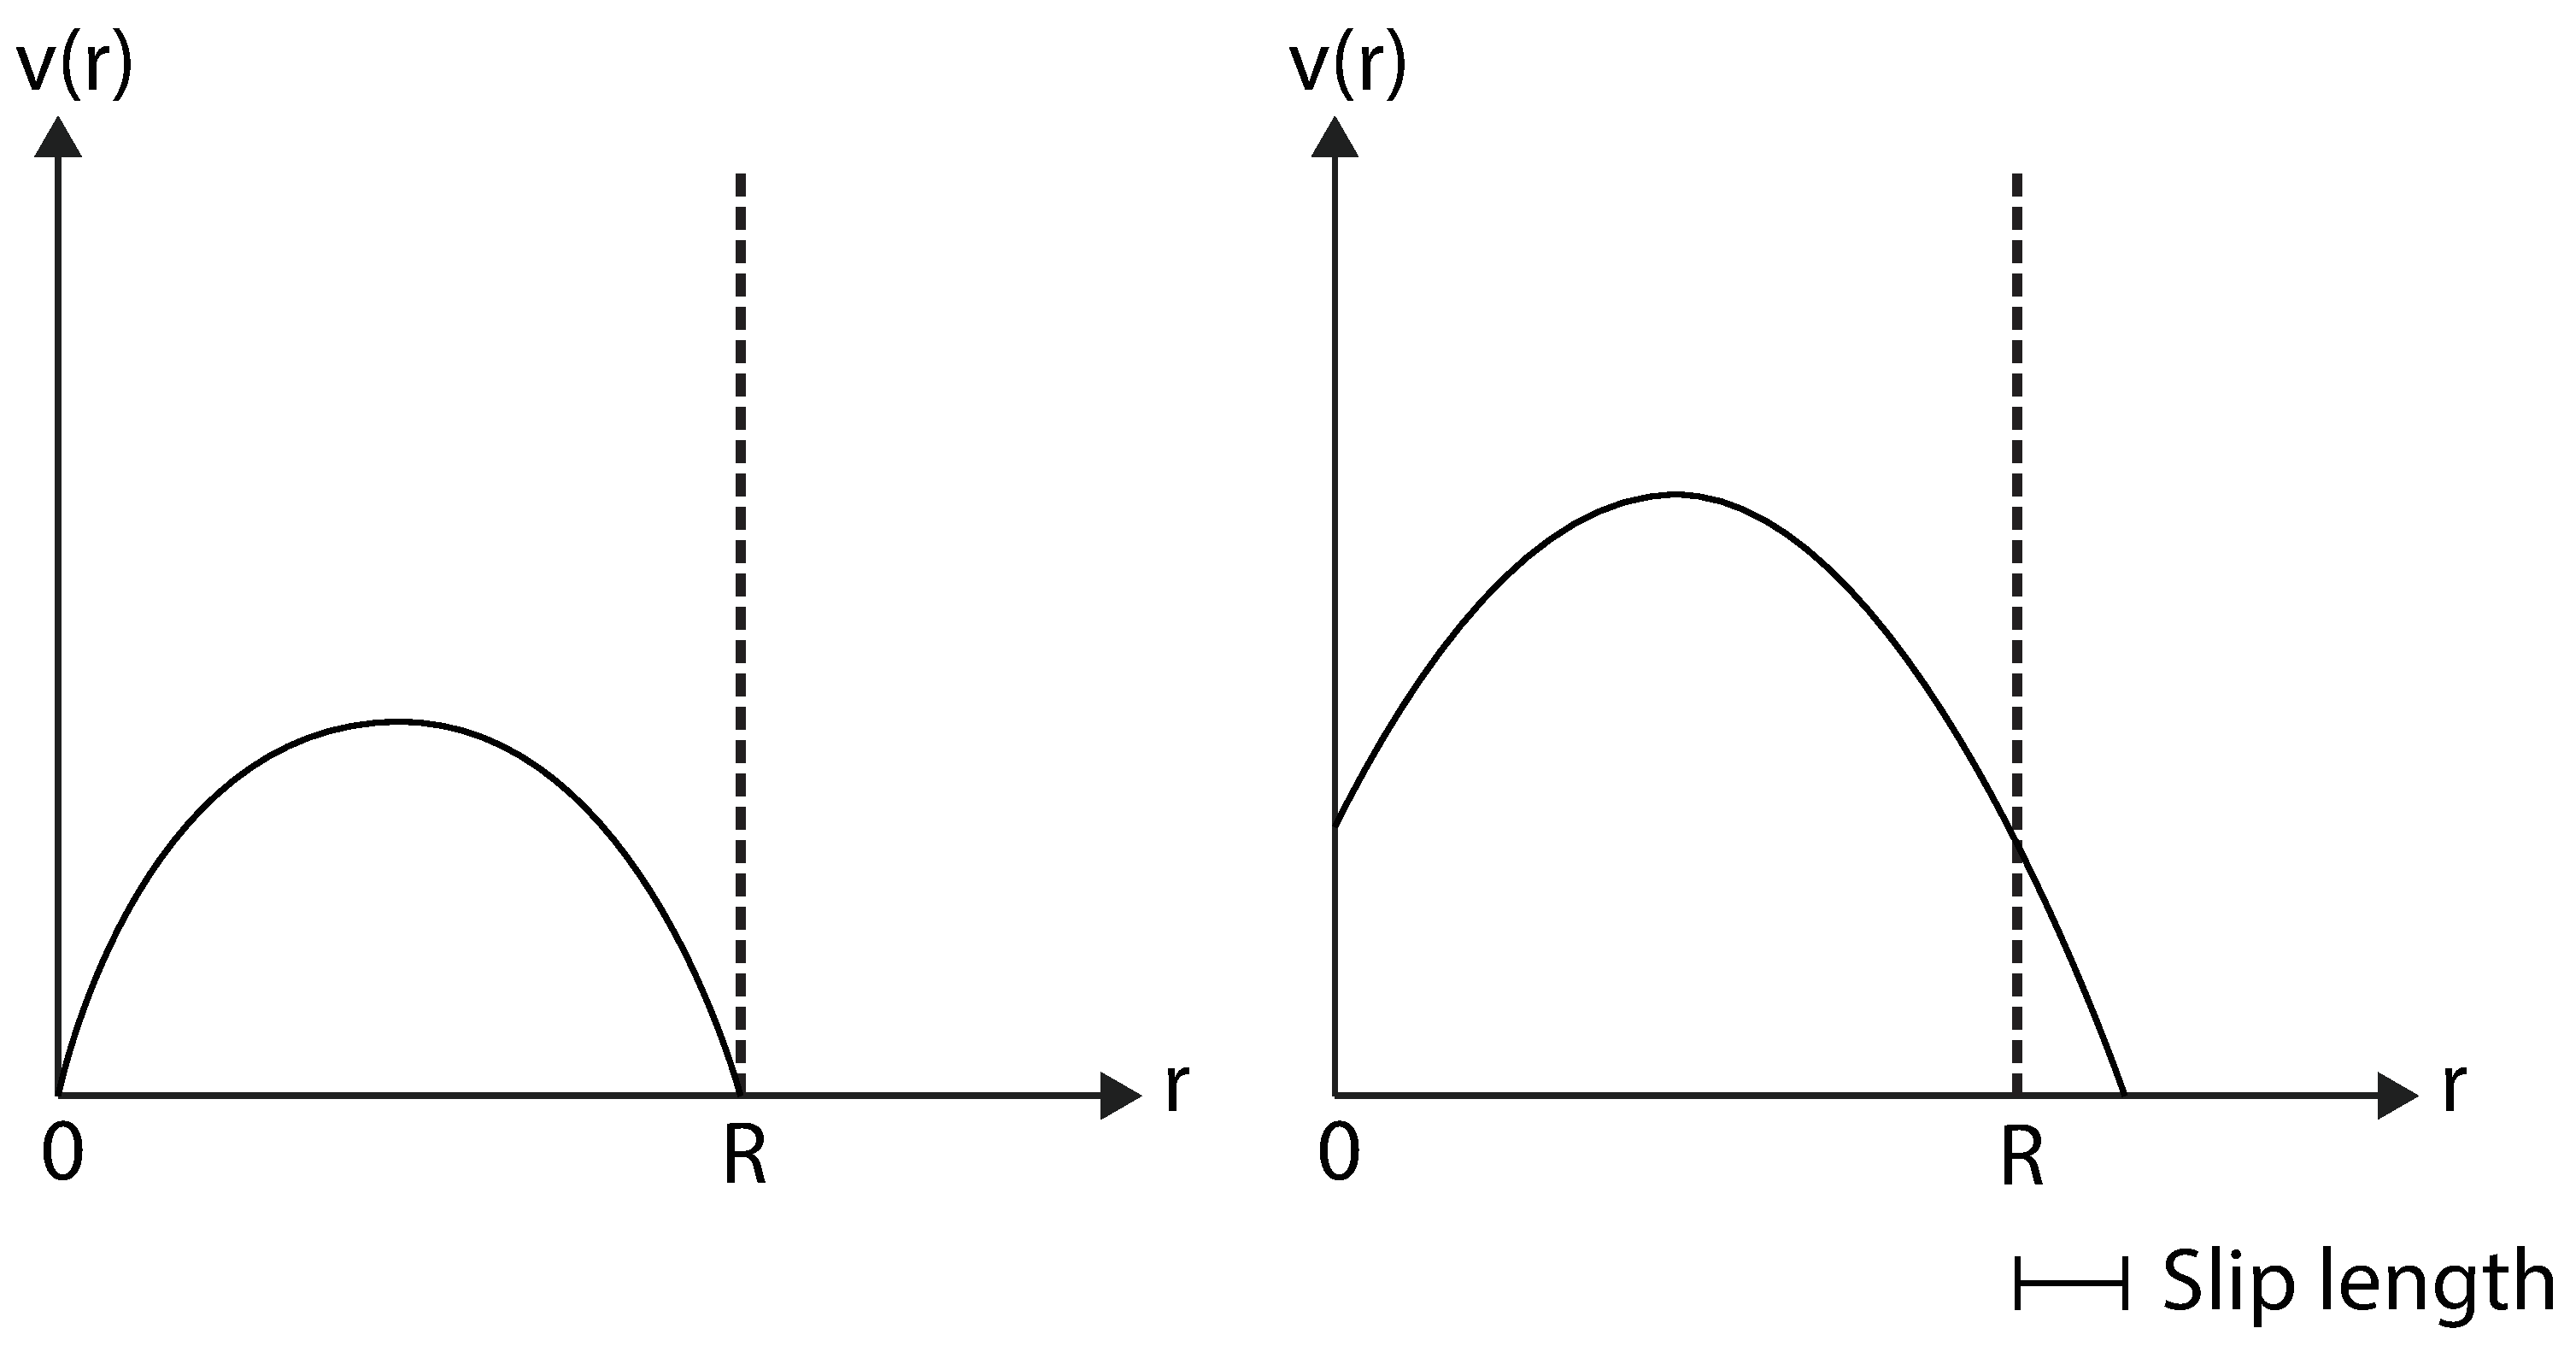
\includegraphics[width=\textwidth, trim=0cm 0cm 0cm 0cm, clip]{DSMC/figures/slip_length.eps}
\end{center}
\caption{Slip length is the distance into the wall we would have to extrapolate a velocity profile for it to reach zero value. We have the no-slip condition on the left, where the slip length is zero whereas we have a non-zero slip length on the right.}
\label{fig:slip_length}
\end{figure}
Maxwell theory predicts the following relation between the slip length and the mean free path
\begin{align}
	\label{eq:noslip_sliplength}
	l_s = \alpha \lambda,
\end{align}
where $\alpha\approx 1.15$ is the slip coefficient \cite{morris1992slip}. The effects of slip velocity become more apparent when the channel diameter is of the same order as the mean free path. By introducing the dimensionless slip length
\begin{align}
	l_s^* = \frac{l_s}{ L} = \alpha \frac{\lambda }{ L} = \alpha \text{Kn},
\end{align}
we see that the ratio of the slip length to the channel diameter is proportional to the Knudsen number. The actual slip velocity (the average velocity of the molecules right next to the wall) can be written as
\begin{align}
	\label{eq:linear_slip_velocity}
	v_{\text{wall}} = \alpha\lambda\frac{\dm v}{\dm n},
\end{align}
where $n$ is the direction normal on the wall\cite{klinkenberg1941permeability}. We call this a \textit{first order} slip model since it is contains only the first derivative of the velocity. Higher order models exists and give corrections that are important in nanoporous media (which is defined in section \ref{sec:nanoporous_media}) where the channels that contribute to flow are of nanometer scale. It is convenient to classify different flow regimes 
\section{Flow regimes}
\todo{Discuss flow regimes}
\section{Nanoporous media}
\label{sec:nanoporous_media}
A porous medium is a material with pores and channels (the pore network) available for fluids. See figure \ref{fig:history_porous_media}. 
\missingfigure{Make a sketch of a porous medium.}